\PassOptionsToPackage{unicode=true}{hyperref} % options for packages loaded elsewhere
\PassOptionsToPackage{hyphens}{url}
%
\documentclass[AMA,STIX1COL]{WileyNJD-v2}
% \usepackage[margin=1in]{geometry}
%\usepackage[numbers]{natbib}

\usepackage{amsmath}
%amssymb
\usepackage{chemmacros}
\usepackage{siunitx}
\usepackage{algorithm}
% \usepackage{lmodern}
% \usepackage{ifxetex,ifluatex}
\usepackage{lineno}
% \usepackage{fixltx2e} % provides \textsubscript
% \ifnum 0\ifxetex 1\fi\ifluatex 1\fi=0 % if pdftex
%   \usepackage[T1]{fontenc}
%   \usepackage[utf8]{inputenc}
%   \usepackage{textcomp} % provides euro and other symbols
% \else % if luatex or xelatex
%   \usepackage{unicode-math}
%   \defaultfontfeatures{Ligatures=TeX,Scale=MatchLowercase}
% \fi
% use upquote if available, for straight quotes in verbatim environments
% \IfFileExists{upquote.sty}{\usepackage{upquote}}{}
% use microtype if available
% \IfFileExists{microtype.sty}{%
% \usepackage[]{microtype}
% \UseMicrotypeSet[protrusion]{basicmath} % disable protrusion for tt fonts
% }{}
% \IfFileExists{parskip.sty}{%
% \usepackage{parskip}
% }{% else
% \setlength{\parindent}{0pt}
% \setlength{\parskip}{6pt plus 2pt minus 1pt}
% }
\usepackage{hyperref}
\hypersetup{
            pdftitle={Solution of Differential Algebraic Equations with Local Constraints on the Latent Space of an Autoencoder},
            pdfauthor={Alejandro Francisco Queiruga},
            pdfborder={0 0 0},
            breaklinks=true}
\urlstyle{same}  % don't use monospace font for urls
\usepackage{color}
% \usepackage{fancyvrb}
% \newcommand{\VerbBar}{|}
% \newcommand{\VERB}{\Verb[commandchars=\\\{\}]}
% \DefineVerbatimEnvironment{Highlighting}{Verbatim}{commandchars=\\\{\}}
% % Add ',fontsize=\small' for more characters per line
% \newenvironment{Shaded}{}{}
% \newcommand{\AlertTok}[1]{\textcolor[rgb]{1.00,0.00,0.00}{\textbf{#1}}}
% \newcommand{\AnnotationTok}[1]{\textcolor[rgb]{0.38,0.63,0.69}{\textbf{\textit{#1}}}}
% \newcommand{\AttributeTok}[1]{\textcolor[rgb]{0.49,0.56,0.16}{#1}}
% \newcommand{\BaseNTok}[1]{\textcolor[rgb]{0.25,0.63,0.44}{#1}}
% \newcommand{\BuiltInTok}[1]{#1}
% \newcommand{\CharTok}[1]{\textcolor[rgb]{0.25,0.44,0.63}{#1}}
% \newcommand{\CommentTok}[1]{\textcolor[rgb]{0.38,0.63,0.69}{\textit{#1}}}
% \newcommand{\CommentVarTok}[1]{\textcolor[rgb]{0.38,0.63,0.69}{\textbf{\textit{#1}}}}
% \newcommand{\ConstantTok}[1]{\textcolor[rgb]{0.53,0.00,0.00}{#1}}
% \newcommand{\ControlFlowTok}[1]{\textcolor[rgb]{0.00,0.44,0.13}{\textbf{#1}}}
% \newcommand{\DataTypeTok}[1]{\textcolor[rgb]{0.56,0.13,0.00}{#1}}
% \newcommand{\DecValTok}[1]{\textcolor[rgb]{0.25,0.63,0.44}{#1}}
% \newcommand{\DocumentationTok}[1]{\textcolor[rgb]{0.73,0.13,0.13}{\textit{#1}}}
% \newcommand{\ErrorTok}[1]{\textcolor[rgb]{1.00,0.00,0.00}{\textbf{#1}}}
% \newcommand{\ExtensionTok}[1]{#1}
% \newcommand{\FloatTok}[1]{\textcolor[rgb]{0.25,0.63,0.44}{#1}}
% \newcommand{\FunctionTok}[1]{\textcolor[rgb]{0.02,0.16,0.49}{#1}}
% \newcommand{\ImportTok}[1]{#1}
% \newcommand{\InformationTok}[1]{\textcolor[rgb]{0.38,0.63,0.69}{\textbf{\textit{#1}}}}
% \newcommand{\KeywordTok}[1]{\textcolor[rgb]{0.00,0.44,0.13}{\textbf{#1}}}
% \newcommand{\NormalTok}[1]{#1}
% \newcommand{\OperatorTok}[1]{\textcolor[rgb]{0.40,0.40,0.40}{#1}}
% \newcommand{\OtherTok}[1]{\textcolor[rgb]{0.00,0.44,0.13}{#1}}
% \newcommand{\PreprocessorTok}[1]{\textcolor[rgb]{0.74,0.48,0.00}{#1}}
% \newcommand{\RegionMarkerTok}[1]{#1}
% \newcommand{\SpecialCharTok}[1]{\textcolor[rgb]{0.25,0.44,0.63}{#1}}
% \newcommand{\SpecialStringTok}[1]{\textcolor[rgb]{0.73,0.40,0.53}{#1}}
% \newcommand{\StringTok}[1]{\textcolor[rgb]{0.25,0.44,0.63}{#1}}
% \newcommand{\VariableTok}[1]{\textcolor[rgb]{0.10,0.09,0.49}{#1}}
% \newcommand{\VerbatimStringTok}[1]{\textcolor[rgb]{0.25,0.44,0.63}{#1}}
% \newcommand{\WarningTok}[1]{\textcolor[rgb]{0.38,0.63,0.69}{\textbf{\textit{#1}}}}
\usepackage{graphicx,grffile}
\makeatletter
\def\maxwidth{\ifdim\Gin@nat@width>\linewidth\linewidth\else\Gin@nat@width\fi}
\def\maxheight{\ifdim\Gin@nat@height>\textheight\textheight\else\Gin@nat@height\fi}
\makeatother
% Scale images if necessary, so that they will not overflow the page
% margins by default, and it is still possible to overwrite the defaults
% using explicit options in \includegraphics[width, height, ...]{}
\setkeys{Gin}{width=\maxwidth,height=\maxheight,keepaspectratio}
\setlength{\emergencystretch}{3em}  % prevent overfull lines
\providecommand{\tightlist}{%
  \setlength{\itemsep}{0pt}\setlength{\parskip}{0pt}}
%\setcounter{secnumdepth}{0}
% Redefines (sub)paragraphs to behave more like sections
\ifx\paragraph\undefined\else
\let\oldparagraph\paragraph
\renewcommand{\paragraph}[1]{\oldparagraph{#1}\mbox{}}
\fi
\ifx\subparagraph\undefined\else
\let\oldsubparagraph\subparagraph
\renewcommand{\subparagraph}[1]{\oldsubparagraph{#1}\mbox{}}
\fi




% Patch equations to properly generate line numbers for review
\newcommand*\patchAmsMathEnvironmentForLineno[1]{%
  \expandafter\let\csname old#1\expandafter\endcsname\csname #1\endcsname
  \expandafter\let\csname oldend#1\expandafter\endcsname\csname end#1\endcsname
  \renewenvironment{#1}%
     {\linenomath\csname old#1\endcsname}%
     {\csname oldend#1\endcsname\endlinenomath}}%
\newcommand*\patchBothAmsMathEnvironmentsForLineno[1]{%
  \patchAmsMathEnvironmentForLineno{#1}%
  \patchAmsMathEnvironmentForLineno{#1*}}%
\AtBeginDocument{%
\patchBothAmsMathEnvironmentsForLineno{equation}%
\patchBothAmsMathEnvironmentsForLineno{align}%
\patchBothAmsMathEnvironmentsForLineno{flalign}%
\patchBothAmsMathEnvironmentsForLineno{alignat}%
\patchBothAmsMathEnvironmentsForLineno{gather}%
\patchBothAmsMathEnvironmentsForLineno{multline}%
}



% \makeatletter
% \def\fps@figure{tbph}
% \makeatother


\title{Solution of Differential Algebraic Equations with Local Constraints
on the Latent Space of an Autoencoder}
\author[1]{Alejandro Francisco Queiruga*}
\address[1]{\orgdiv{Energy Geosciences Division}, \orgname{Lawrence Berkeley
    National Laboratory}, \orgaddress{\state{CA}}, \country{USA}}
\corres{*\email{afqueiruga@lbl.gov}}

\received{\today}
\revised{\today}


\begin{document}

\abstract[Abstract]{
  Multiphase simulation is hard.
Our proposed method is motivated by the problems of multiphase reaction and
transport, where the underlying constraints are the ill-behaved material
properties which are difficult to describe.
Our proposed approach is to build upon modern machine learning
techniques to aid in equation discovery. An autoencoder is trained on
the original material dataset to learn a lower-dimensional
representation of the underlying manifold. The model is designed to be
directly incorporated into a macroscale simulation of physical balance
laws, where now the traditional partial differential equations are being
solved on the learned latent space.
We train an autoencoder to determine the lower-dimensional
representation of the EOS surface using modern deep learning techniques
without using any phase labels. The decoder end of the model is then
plugged back into the balance laws, eliminating the constraint equation.
This provides a more robust
numerical algorithm, while putting the onus of programming part of the
simulation itself onto the computer: tens of thousands of lines of human
written code consisting of theoretical relations, empirical fits, and branching logic are
replaced by code generated by the learned model. The methodology will
first be demonstrated on datasets based on thermodynamic intensive
variables, which are already challenging to analyze, before being
extended to richer datasets such as experimental images or molecular
dynamics. We stress that the proposed approach is only utilizing machine
learning on material data: the simulation is indeed solving physical
balance laws. Through deep learning approaches combined with
domain-specific goals, we can learn representations that are both
interpretable and directly apply to analyzing larger systems.
We illustrate the methodology on two traditional problems: 1) the
pendulum, and 2) the continuous stirred tank reactor.}

\jnlcitation{\cname{Queiruga, A.}\ctitle{Solution of DAEs on Latent Spaces},\cjournal{I. J. Num. Meth. Eng.}, \cvol{2019;00:1--2}}

\keywords{Class file; \LaTeXe; \emph{Wiley NJD}}

\maketitle

\begin{center}\rule{0.5\linewidth}{\linethickness}\end{center}

\hypertarget{header-n3216}{%
\section{Introduction}\label{header-n3216}}

Representing complex physical systems with multiple species, phases,
chemical reactions, and heterogenous scale effects poses an
intractability problem to modeling. How do we analyze complex
experimental data and \emph{ab initio} simulations and derive new
macroscale relations to describe the systems? How do we then implement
these relations in the rest of our analyses and production-scale
computer simulations
Accurately simulating multispecies reaction and transport with
undergoing phase transitions is a critical aspect to a variety of
problems.
This work is motivated by addressing challenges in the simulation of subsurface energy systems, such as shale
and oceanic natural gas reservoirs or engineered geothermal
systems.

Our fundamental goal is to develop the tools
for unsupervised representation learning in way where the
representations have physical and useful meaning.
How can we find a latent space that is good for our tasks?
How can we find regressions in a deep learning context of high enough
accuracy with needed qualities?
How do we include these types of machine-generated models into a
scientific and engineering calculation without sacrificing accuracy?
Can this improve our workflow?
Can we then find paths in the learned space that follow physical laws?


The system of equations we are looking at are, for only two components,
\begin{align}
  \partial_t \rho_{H_2O} =& \nabla \cdot F_{H_2O} + s \\
  \partial_t \rho_{CO_2} =& \nabla \cdot F_{CO_2} + s \\
  \partial_t e =& \nabla \cdot F_{heat} + s
\end{align}
More species add more balance laws (rows of equations). The applications also involve continuum
mechanics and chemical reactions, which are not considered. The interplay of deformations,
reactions, and phase transitions makes the equations extremely difficult
to solve \cite{queiruga_simulation_2019}. 
(In this paper, we use $\partial_t$
and $\dot{()}$ to denote differentiation with respect to time
for compactness.)
The complexity is hidden inside the relationships between temperature
$T$, and pressure,$p$, density, $\rho$, and internal energy $e$ (or
enthalpy, $h$, s.t. $e=\rho h - p$), 
for the materials in question.

% {\bf RESERVOIR PHYSICS LIT REVIEW HERE; Other applications;
% plasticity, }
One of the simulators with the widest-encompassing physical modules is
the TOUGH family of solvers that have been developed at Lawrence
Berkeley National Lab.
The methodology is based on a primary variable switching method in 
The simulator of THAT GUY WITH DUAL VARIABLES I MET AT AGU
parameterizes a simplified hydrate system using density and enthalpy
as the primary variables.
Higher order representations of flow are also a problem to tackle
anisotropy and increase the computational efficiency of the spatial
discretization\cite{hannon_enhanced_2018}. 
Multiphase flow was done with finite elements in \cite{yang_fully_2014}.
THAT MORIDIS FEM PAPER SAY MORE ABOUT IT


A single material with multiple phase transitions
is a challenge in of itself, and the descriptions become combinatorially
more complex as species and phases are added. This results in
combinatorially more human labor and combinatorially more code which
tends to involve complex branching logic. The descriptions then pose
numerical challenges when incorporated into macroscale simulations due
to obstacles such as discrete phase state machines and primary variable
switching.
This work only considers the "single beaker" problem; the flow
and transport aspects have similar challenges. (The next stage of this
work will "connect the beakers".)


We redescribed our problem as a differential algebraic equation
with a constraint: the balances of mass and energy are constrained by
the EOS. We can cast the above equation into a basic form for a
differential algebraic equation,
\begin{align}
  z( u, \partial_t u) &= 0 \\
  c(u) & = 0
\end{align}
where, for the equation above, the variable is $u=\{T,p,\rho,h\}$. We will introduce a new way of thinking about constraints as sets of
solutions or observations of possible $u$:
\begin{equation}
c(u)=0 \longleftrightarrow \left\{ u | c(u)=0 \;\text{or}\; u\; \text{observed} \right\}
\end{equation}
This maps directly to the original experimental procedure for
determining a constraint equation.

Because the EOS was originally derived from data, a data-driven
approach lends itself in which the EOS is a set of points in
temperature-pressure-density-enthalpy space. (In the multicomponent
cases there are more dimensions.)
We will use this set of possible values viewpoint to train an
autoencoder on the set of $u$ for a latent space parameterized by $q$:
\begin{equation}
u = D(q), \; q=E(u) \;\forall u \in U
\end{equation}
which satisifies
\begin{equation}
  D(q)\in U \forall q.
\end{equation}
We can then write the original equation by
\begin{equation}
z(q,\partial_t q)=0
\end{equation}
The actual meaning of the parameterization is not important, so long as
it can be effectively solved and then \emph{decoded} back to the
physically meaningful quantities.

% {\bf ML LIT REVIEW HERE} % TODO
Representation learning methods such as StyleGAN
\cite{karras_style-based_2018} and Flow/Glow \cite{kingma_glow:_2018} have shown
the ability to find meaningful dimensions in the latent space,
e.g. the popular ability to transform age, race, and gender of human
faces in a smooth way.
But, can this directions be used meaningfully?

Recent review papers have highlighted open applicaitons of machine
learning to subsurface systems \cite{bergen_machine_2019} and
climate scale systems  \cite{reichstein_deep_2019}.
History matching on the latent space of a GAN was demonstrated on a
synthetic geomorphology by Mosser, 2019 \cite{mosser_deepflow:_2019}.

Many approaches try to use machine learning to learn the dynamics of a
system.
The method of Dynamic Mode Decomposition
to learn a linear operator based on time series data \cite{tu_dynamic_2014,kutz_dynamic_2016}. 

Extending this space with known features, such as partial derivatives,
\cite{ one of kutz's students}
Our presented approach differs from this approach by saying that we
know the dynamics {\em a priori}, but do not how to represent the
current state in a useful way. (Our approach will be later extended to
learn dynamics in a second step using the learned representation as a
fixed input.)

\cite{wu_physics-informed_2018}
\cite{xie_tempogan:_2018}

 A program synthesis approach was used to search for and evaluate
 possible methods of Peridynamics in Queiruga, 2017
 \cite{queiruga_numerical_2017}. (An open source implementation of the
 study can be found Periflakes\cite{queiruga_periflakes_2019} using the
 Popcorn/Cornflakes system for symbolic code generation
 \cite{queiruga_cornflakes:_2018,queiruga_popcorn:_2018}.)

Part of the new modern software engineering framework involves replacing
human-written code with computer-written code. We are applying this
mindset from industry problems in the artificial
intelligence space into scientific computing.


This work proposes a new methodology that steps away from the
traditional approaches. 
In this approach, we directly \emph{look for solvable representations}
instead of representations that carry human intuition. We value
simulation runtime and robustness. Further, we must remember the value
of the human effort involved: beyond improving computational aspects,
we are fully automating part of the human involvement in programming
the simulator.

There are infinitely many representations of a system. The simplest and clearist description is not neccessarily the best way
to solve it, and vice versa.


We demonstrate this approach to solving constrained differential
equations on the pendulum, before demonstrating two EOSes of water: one
with just liquid-gas phases, and one with liquid-gas-ice-supercritical
regimes. The notion of phases does not appear in this multiphase
simulation. We show a model architecture that is able to learn phase
labels in the unsupervised autoencoder training process, such
human-scientist interpretable results are obtained from the machine
learning process. We compare this and other model architectures,
including common deep neural networks, based on autoencoder error and
simulation success metrics. We stress that the presented approach is
only utilizing machine learning on material relations derived from
empirical data: the simulation is indeed solving physical balance laws.

We build a dataset using the IAPWS solutions. The proposed
methodology applies to experimental data directly, or preexisting
compendiums of empirical fits and theoretical relations.
Note that, even if a relation can be theoretical derived, that does
not mean that the analytical relationship yields the best program
implementation: it is often the case that numerial approximations are
superior to closed-form mathematical solutions in computational
efficiency, accuracy, and numerical stability.

In Section 2, the balance of mass and energy will be described for a
single multiphase material. We will discuss the current state of the
art algorithm for deriving relationships for multiphase materials, and
then the primary-variable switching algorithm that is used in
state-of-the art solvers. The equation will then be recast as a
constraint problem in th above form.
In Section 3, we will demonstrate applying the autoencoder learning
methodology to solve the pendulum,
which can be considered the archetypical constraint problem.
In Section 4, the autoencoder methodology wil lbe applied to the
equation of state of water. In Section 5, the new simulation process
will be described, wherein the learned decoders are placed into the
balance laws, forming newly discovered equations on learned
representations. The software implementation of the training and
simulation programs are detailed in Section 6. The new simulation
framework on sets of learned representations is evaluated on
multiple datasets of varying extents of water with a
hyperparameter search on a suite of test problems to prouce the discussion of Section 7, as
well as a systematic automated testing procedure of a
machine-dominated programming methodology.
Active research and software development directions are
concluded in the final section.

The notebooks and software implementations are released open source to
accompany this work. They can be found at the github repository
located at: \href{https://github.com/afqueiruga/latentsim}.
Certain components are factored into submodule repositories which are
each released under the LGPL at seperate repositories referenced in
the implementation details.

\section{Multiphase Equations of State}


For this preliminary work, we consider only a single-beaker problem
without flow, the idealization of the continuous stirred-tank reactor (CSTR), as illustrated
in Figure \ref{fig:cstr}. 
In the analysis of geological fluids, this idealization is used in the
assumption of well-mixed pore spaces at the macroscale.  Let \(\rho\)
be the material density, measured in \si{kg/m^3}; \(T\) be the
temperature, measured in \si{K}; \(p\) be the material pressure,
measured in \si{Pa}; \(h\) be the material
specific enthalpy, measured in \si{J/kg}; and \(u\) be the internal
energy, measured in \si{J/kg}, and related to the enthalpy by  \(\rho u = \rho h - p\). There are two equations for
balance of mass and energy.
\begin{align}
\partial_t \rho & = \mathbf{k}_p(p_\infty - p) + r\\
\partial_t \rho u & = \mathbf{k}_T(T_\infty-T) + s + h q_{mass}
\end{align}
The beaker is exposed to a reservoir with \(p_\infty\) and \(T_\infty\)
via a mixed boundary condition straw with transport and conduction
coefficients \(\mathbf{k}_p\), \(\mathbf{k}_T\). 
We are neglecting upstreaming in the connection between the reservoir
and the container. Mass and heating
sources and sinks are the terms \(r\) and \(s\).


\begin{figure}
  \centering
  \includegraphics[width=3in]{../figures/cstr_vector.pdf}
  \caption{ \label{fig:cstr} Illustration of the Continuous
    Stirred-Tank    
  Reactor. The material in the reactor is exposed to a reservoir with
  pressure
  $p_\infty$ and temperature $T_\infty$ via a conduit with permeability
  and thermal conductivities $k_p$ and $k_T$, direct forced mass
  injection or withdrawal $r$ via a pump, or heating and cooling $s$
  via a heater/heat-exchanger. Stirring and insulation keeps the
  material at a uniform pressure and temperature. Gravity is
  neglected (though is usually the motivation for putting a feeding inlet at
the top and product outlet at the bottom.)}
\end{figure}

We also consider the phase equilibria: beyond the scale of resolving
individual bubbles, it is possible
for a control volume to be a mixture of multiple coexisting
phases.
(For a very fine scale simulation, e.g. at the pore scale, bubbles
would be explicitly modeled.)
We introduce a saturation $S_{phase}\in[0,1]$ for each phase;.
The material can exist on this section of the surface as a mixture of
the two phases. Thus, its density is calculated by a mixing the
properties of all phases at that point in the phase diagram:
\begin{align}
  \rho = & S_{gas} \rho_{gas} + S_{liq} \rho_{liq} + S_{ice}
  \rho_{ice} + S_{crit} \rho_{crit} \\
  \rho h =& S_{gas} \rho_{gas} h_{gas} + S_{liq} \rho_{liq} h_{liq} + S_{ice}
  \rho_{ice} h_{ice} + S_{crit} \rho_{crit} h_{crit}
\end{align}
Each phase
and equilibrium surface constrains the possible saturations. For example, on the boiling equilibrium surface there are two phases with some mixture
saturations \(S_{gas}=1-S_{liq}\) and $S_{ice}=S_{crit}=0$. 
For water, three phases can exist in equilibrium. Given more species, it is possible for an arbitrary number of phases
to be in equilibrium; there is a quadruple point in methane-water
hydrates.

Note that the definition of enthalpy as a per-mass quanitity means the mixture needs to be weighted by the
density: $h_{mix}=\sum{\rho_a h_aS_a}/\sum{rho_aS_a}$.

But, what is a phase boundary? The traditional explanation is shown in
Figure \ref{fig:phaseboundaries}. The use of intensive properties breaks down:\footnote{https://en.wikipedia.org/wiki/Phase\_transition}

\begin{quote}
Phase transitions occur when the thermodynamic free energy of a system
is non-analytic for some choice of thermodynamic variables (cf. phases).
\end{quote}


{\bf Remark:} This interpretation breaks down with the existenceof super-saturated phases in non-stable regions: e.g., it is possible to
heat water beyond it's boiling point in a microwave. We are concerned
with environments where this would not happen (the very rough and
heterogenous) pores of rocks, so we have not thought of how to
integrate this problem.

\subsection{Forms of Equations of State}

This work focuses on the EOS of pure water. The most accurate
formulations were developed by the International Association for the
Properties of Water Steam (IAPWS) using a variety of experimental
sources for multiple phases \cite{wagner_iapws_2000,
  water_revised_2007, water_revised_2009}. We utilize the 1997
formulation for water gas, liquid, and supercritical phases, and the
2006 formulation for the Ice Ih phase to build the dataset.\footnote{Our
implementation is publicly available at GITHUB:EOS.} (Their
painstaking work in determining the forms of decent fits is a great
motivation for a 21st century approach.)
We can also assemble the surface of possible $T,p,\rho$ coordinates,
shown in Figure \ref{fig:pTrho}.
\begin{figure}
\centering
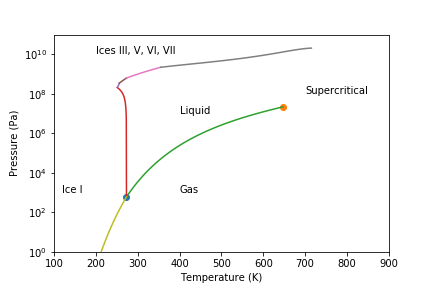
\includegraphics[width=4in]{../figures/phase_diagram.png}
\caption{\label{fig:phaseboundaries}Phase boundaries for water on the $T-p$ diagram. The standard
interpretation is that the properties of the material change
drastically when crossing this boundary. Note how it is possible to form a path from a
definitively gas state to a definitively liquid state without crossing
a phase boundary. The supercritical regime has no clear boundaries,
but requires a separate curve fit in practice due to numerical challenges.}
\end{figure}

\begin{figure}
\centering
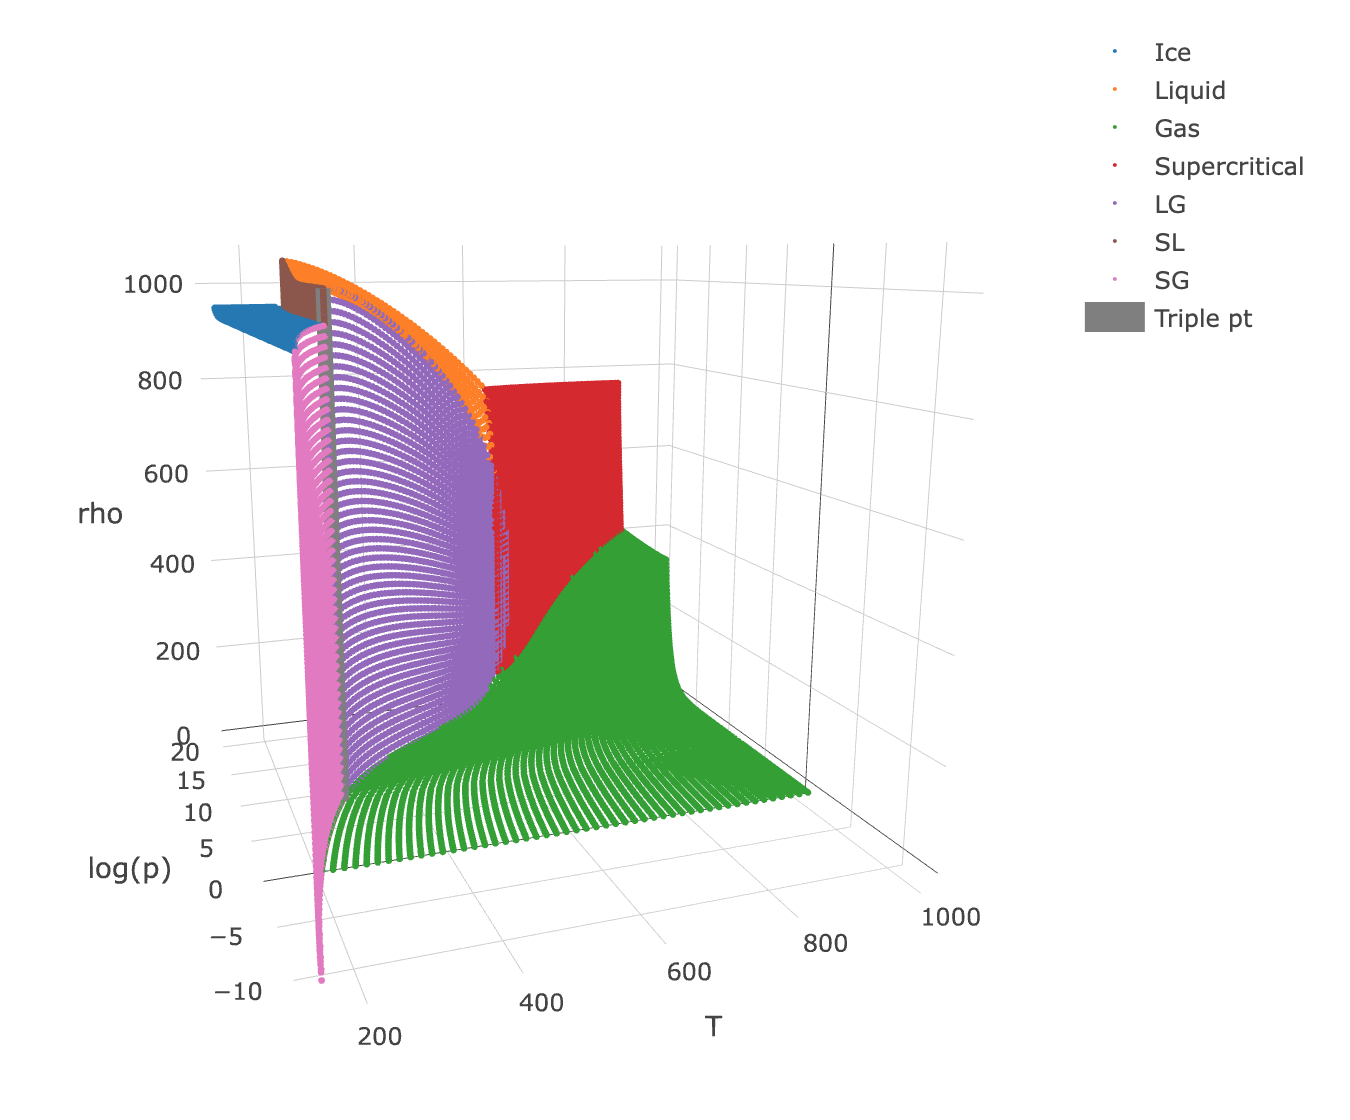
\includegraphics[width=4in]{../figures/water_eos.png}
\caption{\label{fig:pTrho} The $\log{p}$, $T$, $\rho$ equation of
  state surface for water in units of $\log{\text{Pa}}$, K, and \si{}{kg/m$^2$} This plot spans four phases, three
  equilibria, and the triple point, which are each given their own color.
  There is a fourth dimension to the surface of enthalpy $h$ that exhibits
  similar discontinuities; the $\log{p}$, $T$, $h$ surface is plotted
  in the Appendix. (Every point on this plot is a point in the
  generated dataset used for the optimization.) An interactive version
of this figure is included online.}
\end{figure}


{\bf Remark:} There are even more known phases of crystal ice which for water
For water, the supercritical phase only occurs at extreme conditions
near the mantel or near magma chambers, which could be potential sites
for geothermal plants\cite{elders_science_2010}. The exotic ices only occur in
laboratory conditions\cite{water_revised_2009}. For our case, we only handle the Ice I and cutoff the
regime at \si{10^8}{Pa}. For other materials these exotic phases can be
applicable. Methane $CH_4$ is actually well beyond its supercritical
point at T=\si{-82.59}{C}\cite{the_engineering_toolbox_methane_2008}, so only an appropriate gas law can do the trick, until
the bi-species hydrate phase comes into play. Handling the
liquid-gas-equilibrium-supercritical state transition also comes into
play with other fluids; for example, in geoengineered systems using
$CO_2$ such as geothermal plants and carbon sequestration facilities, the
working fluid is often in the supercritical regime at depth, and the
phase boundary \cite{pruess_feasibility_2006,oldenburg_migration_2006}. 
When binary mixtures are involved, the number of possible phases and
equilibria increases again; methane hydrate simulators have 15
states \cite{moridis_simulation_2019}.


{\bf Remark:} Many popular forms of EOS do not even have closed form
expressions. The family of cubic equations of state for nonideal
gases, such as the Peng-Robinsion equation \cite{peng_new_1976}, are
expressed as functions for $p$ of $V$ (a proxy for $\rho$) and
$T$. Since $\rho$ is rarely a primary varibale, these expressions must be inverted for
$\rho$ given $p$ by solving the cubic equation. This can be performed
analytically, as is done in TOUGH+, but often polynomial roots can
be best solved numerically. When the equations become more
complicated, such as when there are gas mixtures, the equations of
state must be solved numerically. TOUGH+ employs a Richardson
iteration \cite{moridis_users_2014-2}.
Note how this is a numerical
iteration {\em inside} of another numerical iteration that is trying
to differentiation this equation state. Approximations
abound--the mathematical theory is not straight foward. Passing
automatic differentiation objects through these computations is
difficult in practice. Equations are
often solved faster and more accurately by numerical
approximations--why not completely rewrite the equations?

{\bf Remark:} The relations inside of EOSes are often artificially
smoothed. For example, the hydrate equilibrium surface has a kink at
the ice-liquid phase boundary in water. This causes problems
numerically when a material state is moving along this equilibrium, so
it is artificially smoothed using splines or the hyperbolic tangent to
improve convergence in TOUGH+Hydrate \cite{moridis_users_2014}. Approximations abound. 


\hypertarget{header-n3253}{%
\subsection{State Machine logic}\label{header-n3253}}


The typical methodology is to use the empirical relations for density
and enthalpy \(h\) as a function of pressure and temperature and solve
the DAE for \(p\) and \(T\) implicitly:
\begin{align}
\text{Solve for}\, p(t)\, \text{and}\, T(t)\, \text{such that:}\\
\partial_t \rho(p,T) & = \nabla \cdot \mathbf{k}\nabla p + r\\
\partial_t \rho(p,T) h(p,T)-p & = \nabla \cdot \mathbf{k'}\nabla T + s
\end{align}
The complication is that the functions \(\rho(p,T)\) and \(u(p,T)\)
are not well defined functions due to the presence of phase changes that
yield sharp discontinuities in \(p,T\), as shown in Figure 1 for
water.
Each state requires a potentially different set of primary
variables. For a pure water system, this would have to be:
\begin{center}
\begin{tabular}{l|c|c}
  State & $X_1$ & $X_2$ \\
  \hline
  Ice & $p$ & $T$ \\
  Liquid & $p$ & $T$ \\
  Gas & $p$ & $T$ \\
  Supercritical & $\rho$ & $T$ \\
  Ice-Liquid & $S_{ice}$ & $T$ \\
  Ice-Gas & $S_{ice}$ & $T$ \\
  Gas-Liquid & $S_{gas}$ & $T$ \\
  Ice-Gas-Liquid & $S_{ice}$ & $S_{gas}$ 
\end{tabular}
\end{center}
Solving the balance laws with this caveat requires the incorpoeration
of a statemachine. Representing the material with the known
representations thus requires two variables and an additional state
tag. For the complete states of water, the states and their possible
transitions is shown in Figure \ref{fig:statemachine}.
  \begin{figure}
    \centering
    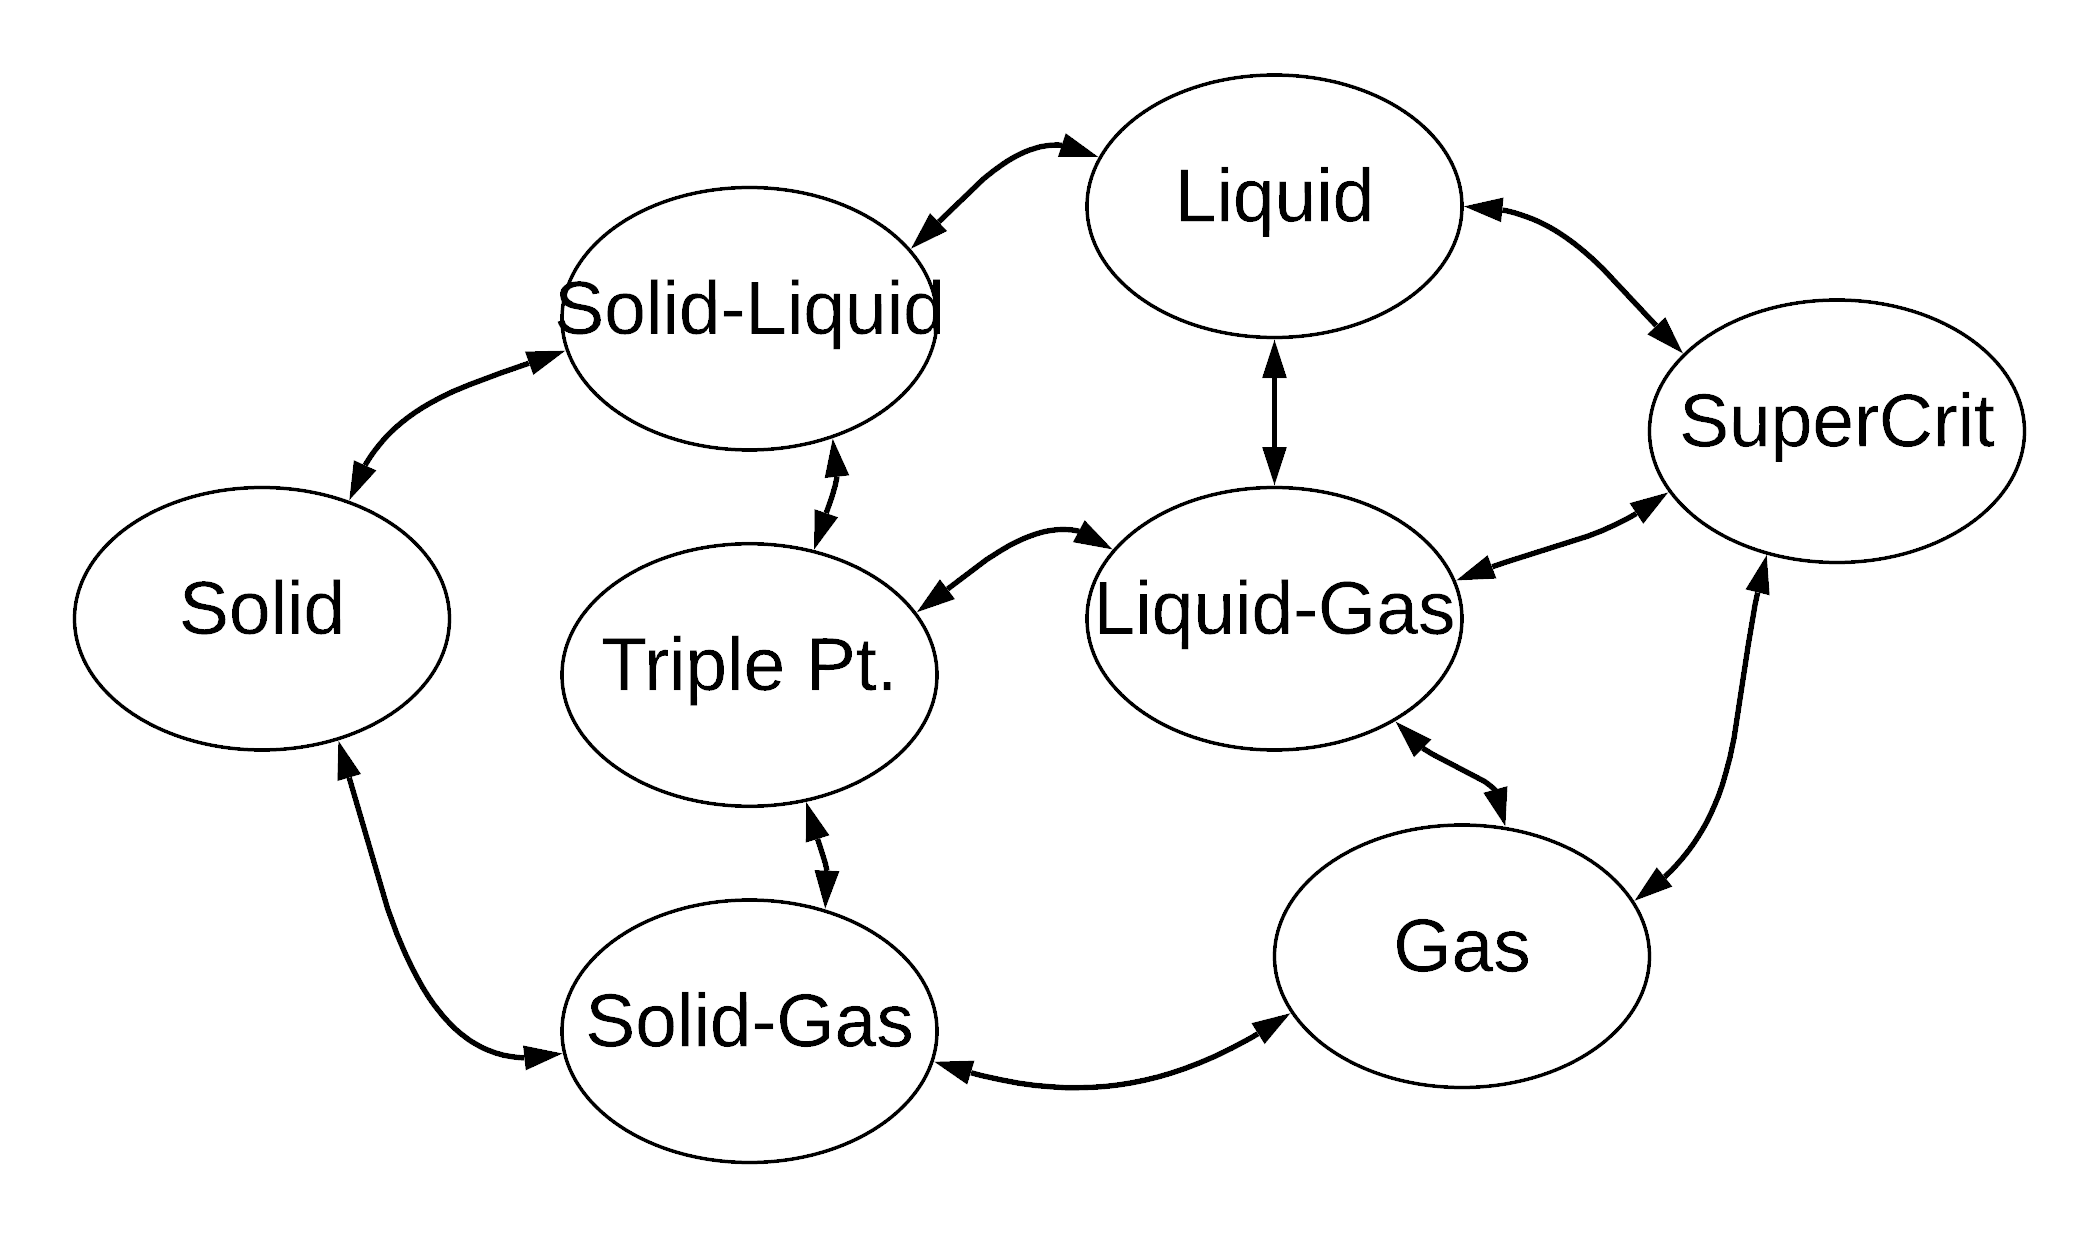
\includegraphics[width=4in]{../slides/phase_4.png}
    \caption{\label{fig:statemachine}States and possible transitions for water.}
\end{figure}
Formulate balance equations as
\begin{equation}
R(X ; phase) = 0
\end{equation}
Solve the differentiable part:
\[\frac{\partial R}{\partial X}\Delta X^{k+1/2} = -R(X^k ; phase^k)\]
and iterate on the nondifferential part:
\[phase^{k+1},X^{k+1} = statemachine(X^{k+1/2} ; phase^k)\]
The phase switching logic has the form of a switch case illustrated in
Algorithm \ref{alg:statemachine}.

 
\begin{algorithm}
\begin{lstlisting}[caption={Finite State Machine transition logic}, label={alg:statemachine}]
switch phase_old:
  case gas:
    if p,T crossing boundary:
      phase_new = liquid_gas
  case liquid:
    if p,T crossing boundary:
      phase_new = liquid_gas
  case liquid_gas:
    if S_gas >= 1:
      phase_new = gas
    if S_liquid >= 1:
      phase_new = gas
\end{lstlisting}
\end{algorithm}
%  \begin{verbatim}

%\end{verbatim}

\hypertarget{header-n3262}{%
\subsection{A constrained Differential Algebraic
Equation}\label{header-n3262}}

We argue that the relations that are used are not the \emph{ground
truth} in of themselves. Beyond ideal gases and simple linear fluids,
the functions \(\rho(p,T)\) or \(p(\rho,T)\) are simply complicated fits
that were derived in an ad-hoc piecewise fashion from experimental data.
This is not a bad thing---it is the fundamental nature of the problem.
When we look at the corpus of literature on a material as water, what we
actually have is a decision branch to multiple different complicated
fits for each material branch.

We instead replace our problem with two balance laws and one unknown
constraint:
\begin{align}
\text{Solve for}\, \rho(t), \, h(t), \, p(t),\, \text{and}\, T(t)\,
  \text{satisfying:} \nonumber
                       \\
\partial_t \rho &  = \mathbf{k}_p(p_\infty - p) + r\\
\partial_t (\rho h-p) & = \mathbf{k}_T(T_\infty-T)  + s + h\left(\mathbf{k}_p(p_\infty - p) + r\right) \\
\text{such that they lie on the material EOS,}\nonumber
                                                \\
  \rho,h,p,T & \in \{\text{EOS}\}\\
  \text{given }\rho,h,p,T \text{ at } t=0. \nonumber
\end{align}
The \emph{ground truth} is the experimental data in the first place; the
branching curve fit is only one realization of representing the data. We
have demonstrated that it is not possible to represent any two of these
in terms of the other two; and even if so, it is not necessarily a good
and robust fit. What if we search for a new fit?

\hypertarget{header-n3267}{%
\section{The Pendulum}\label{header-n3267}}

An archetypical constraint problem is the pendulum. Posed as dynamics
problem with a Lagrange-multipler-esque centripetal force, it
has three unknowns wtih two second-order equations and a constraint,

\begin{align}
\text{Solve for}\, x(t), \, y(t), \, f(t) \, \text{satisfying:} \nonumber \\
m \ddot{x} & = f x/\sqrt{x^2+y^2} \\
m \ddot{y} & = f y/\sqrt{x^2+y^2} - m g \\
  x^2 + y^2 & = R^2
  \text{given } x,y, \dot{x},\dot{y} \text{ at } t=0. \nonumber
\end{align}
Note that we are considering the nonlinear pendulum.

There are many ways to solve this canonical equation: Lagrange
multipliers (\(f(t)\) is the multiplier in the way we have written it
above), penalties, change of variables, etc. The change of variables
method exploits the Lagrangian mechanics formulation, where we state
the Lagrangian,
\begin{equation}
\mathcal{L} = \frac{1}{2}m\left(\dot{x}^2 + \dot{y}^2\right) - m g y
\end{equation}
with the constraint that \(x\) and \(y\) lie on the path.
We can introduce a new variable \(\theta\) that parameterizes
\(x=R\cos\theta\) and \(y=R\sin\theta\) and rederive the equations of
motion with the familiar,
\begin{align}
\text{Solve for}\, \theta(t) \ \text{satisfying:} \nonumber \\
\frac{\mathrm{d}}{\mathrm{d}t} \frac{\partial \mathcal{L}}{\partial
  \dot{\theta}} =
  \frac{\partial \mathcal{L}}{\partial \theta}
   \text{given } \theta,\dot{\theta} \text{ at } t=0. \nonumber
\end{align}
In this example, this lets us collapse the problem into a
single-component second-roder differential equation.

In our methodology, we do not have an explicit equation for the
constraint, but a dataset of $X$ of $(x,y)$ pairs that are on the manifold. For
our proof-of-concept test, we manufacture this data for the circular
pendulum to verify against the analytical solution:
\begin{equation}
y = \left\{ (R\cos\theta_i, R\sin\theta_i)\; | \;\theta_i \in [-5\pi/4,\pi/4] \right\}
\end{equation}
We also try a ``goofier'' looking curve with no known closed form
solution to exercise the methodology.
For the equation of state problem, this is analogous to the dataset
of $p,T,\rho,h$ 4-tuples that make the plot in Figure \ref{fig:pTrho}.

The manifold for this simple problem is smooth, so two nested
polynomials forms the autoencoder:
\[\left\{\begin{array}{c} x\\y\end{array}\right\}
\rightarrow W_{enc} x^n +b_{enc}\rightarrow q \rightarrow W_{dec} x^n +b_{dec}\rightarrow 
\left\{\begin{array}{c} x\\y\end{array}\right\}\]
where $x^n$ denotes a polynomial basis set, e.g. for two variables $x^n=\{x,y,x^2,xy,y^2,..y^n\}$.
(We explicitly write the bias \(+b\); it is equivalent to including
\(x^0=1\) in the polynomial set.) 

We'll use the autoencoder to generate the parameterization of \(x(q)\)
and \(y(q)\). To do this, we optimize the loss function $L$ (a
distinct symbol from the Lagrangian $\mathcal{L}$),
\begin{equation}
L(x) = \left\| x-D(E(x)) \right\|_2^2
\end{equation}

\begin{figure}
  \center
\includegraphics[width=3in]{../figures/autoencoder_balance_detailed.png}
  \caption{\label{fig:balance}Illustration of the insert of the encoder to form the
  description of the system of equation. The equations
  of motion are generated in a declarative programming methodology,
  where the trained decoder can be extracted and inserted into the abstract
  syntax tree, which can then be differentiated and inserted into a
  time stepping loop.}
\end{figure}

The process of learning and generating the code is illustrated in
Figure \ref{fig:balance}.
When we want to solve the dynamics, we can treat the autoencoder the
same as \(x(\theta)\), plugging it into the equation for the Lagrangian,
\begin{equation}
  \mathcal{L}(x(q),v(q,\dot{q}))
\end{equation}
Taking the partial derivatives with respect to the feature variable and
its rate, the components to the equation of motion are build the DAE we know from physics:
\begin{equation}
  \frac{\mathrm{d}}{\mathrm{d}t}\frac{\partial \mathcal{L}}{\partial \dot{q}} =
  \frac{\partial \mathcal{L}}{\partial q}.
\end{equation}
By the chain rule, the velocities are related to the
feature space by
\begin{equation}
\dot{x} = \frac{\mathrm{d}x(q)}{\mathrm{d}t} = \frac{\partial x}{\partial q}\frac{\mathrm{d}q}{\mathrm{d}t}
\end{equation}
and similarly for the \(y\) direction.
Then plug it into a Runge Kutta (trapezoidal) to solve with Newton's
method:
\begin{equation}
\frac{\partial \mathcal{L}}{\partial \dot{q}}_i - \Delta t
\frac{\partial \mathcal{L}}{\partial q}_i = \frac{\partial
  \mathcal{L}}{\partial \dot{q}}_0 + \Delta t \frac{\partial
  \mathcal{L}}{\partial q}_0
\end{equation}

Solutions are shown in Figure \ref{fig:pendulum}.
\begin{figure}
\centering
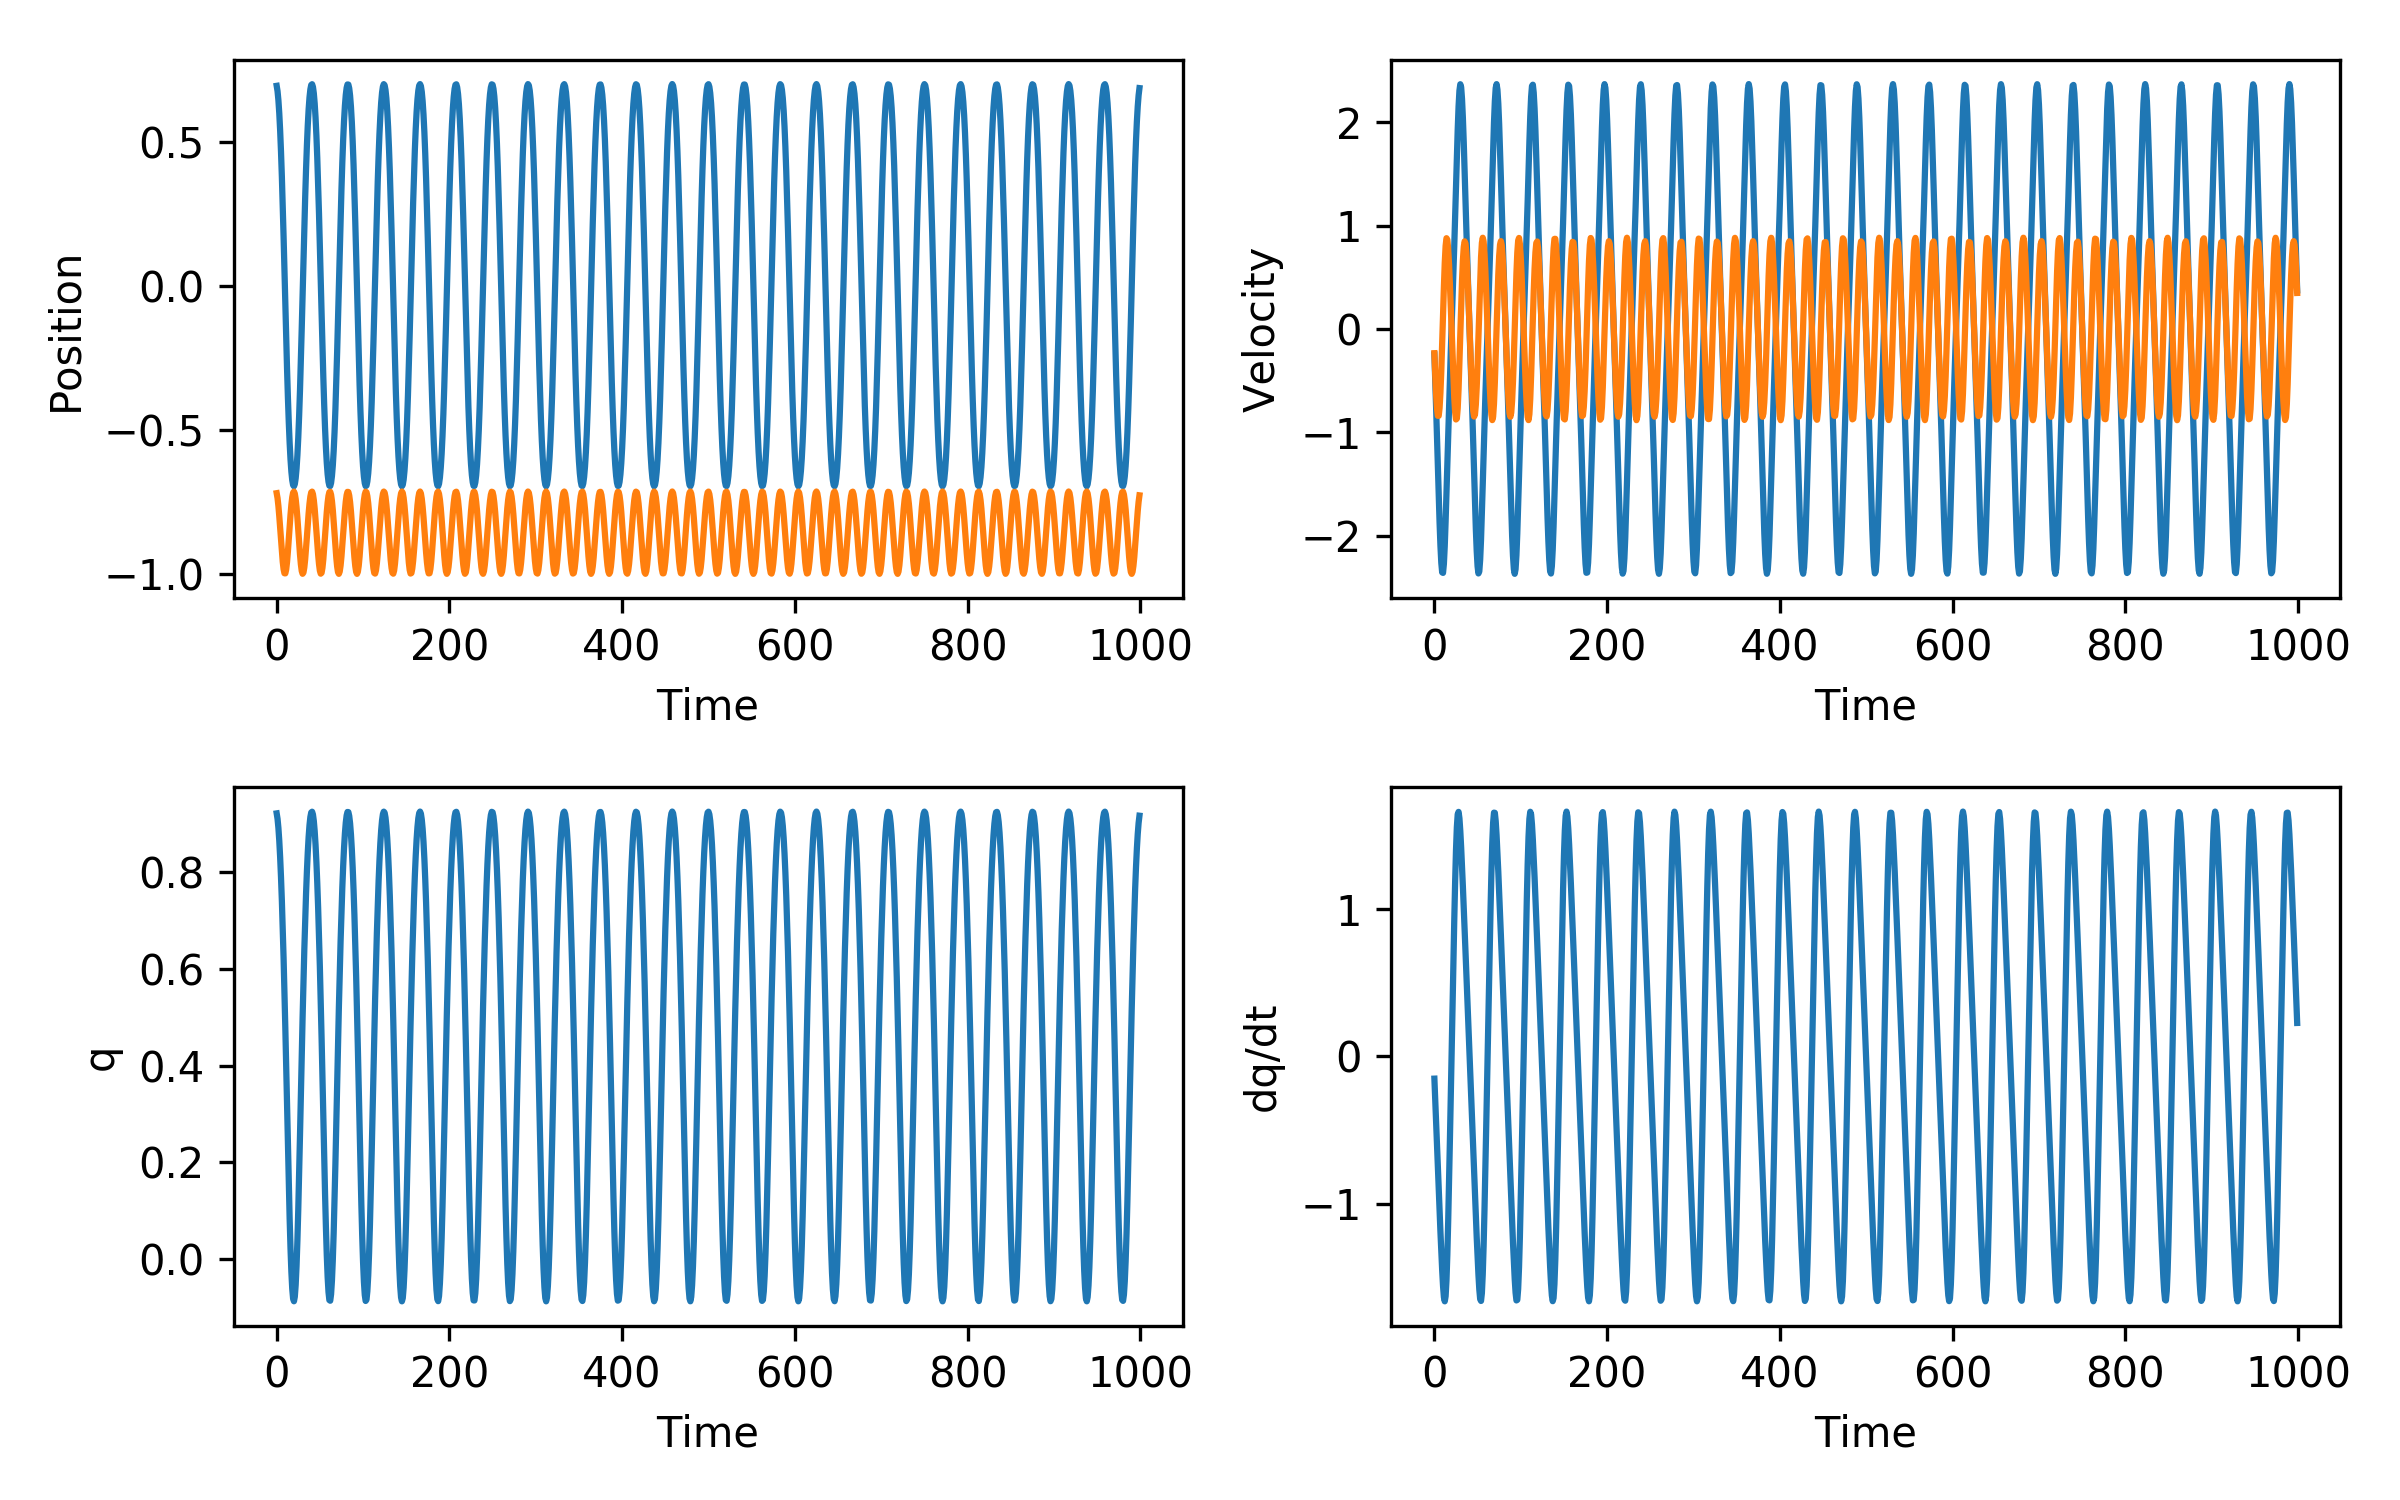
\includegraphics[width=5in]{../figures/pendulum_q.png}
\caption{\label{fig:pendulum}Solution of the pendulum on an arbitrary latent space.}
\end{figure}

\hypertarget{header-n3294}{%
\section{Representation Learning for
Reparameterization}\label{header-n3294}}

The central idea of this work is to obtain two new variables solve for
those directly which have no physical meaning other than simply being a
parameterization of the equation of state constraint. We want to select a
\(q_1\) and \(q_2\) to require no auxilary phase index to define the system
and no additional logic in the code. The sharp kinks and possible
discontinuities can be a part of the functions
\(\rho(q_1, q_2), p(q_1, q_2), h(q_1, q_2)\) and \(T(q_1, q_2)\).


\hypertarget{header-n3299}{%
\subsection{Latent Space}\label{header-n3299}}

Instead of the painstaking work of parameterizing phase boundaries and
determining curve fits by hand, we rephrase the problem of representing
the equation of state by learning and autoencoder. We have an encoding
phase, \(E(\rho,p,e,T; a)\) and a decoding phase, \(D(u,v; b)\) that
forms an identity function with a compressed subspace:
\begin{equation}
\left\{ \begin{array}{c}
T\\ p\\ \rho\\ h
\end{array}\right\} \rightarrow  E \rightarrow 
\left\{ \begin{array}{c} q_1\\q_2 \end{array} \right\}\rightarrow D \rightarrow 
\left\{ \begin{array}{c}
T\\ p\\ \rho\\ h
\end{array}\right\}
\end{equation}
The autoencoder is solved for by optimizing its parameters using the
goal

\begin{equation}
\min_a \sum_x \left( x - D(E(x;a);a) \right)^2
\end{equation}

Note that we are not yet considering constraints \(c\) with partial
differential equation components in space. These types of material
equations of states are only enforced pointwise. The time components of
the equations can contain spatial derivatives; i.e. this method fits
easily inside a finite volume simulation with little change.

\hypertarget{header-n3305}{%
\subsection{Training}\label{header-n3305}}

We use a Euclidean norm loss function with a contractive penalty:

\[L(x)=\left\|x-D(E(x))\right\|^2_2+\lambda\left\|\frac{\partial E}{\partial x}\right\|_F^2\]

The gradient on the encoder is a \(4\times2\) matrix in our case, and
\(\|\|_F\) denotes the Frobenius norm. The contractive penalty
\(\lambda\) smooths out and evenly distributes the mapping to \(q\).

The variational autoencoder is a little more complicated to implement,
and we do not necessarily want to match a Gaussian interior. Because we
generated our datasets artificially (both in this manufactured setting
and in an actual laboratory setting), the dataset does not reflect draws
from a distribution, so the KL divergence against a gaussian is not
quite applicable.

We note that penalizing the decoder would smooth out the sharp kinks at
phase boundaries.

The dataset is split into a standard $2/3-1/6-1/6$ division into
training-testing-validation groups. We note that we can always
manufacture more datapoints. We train by alternating phases. The first
step is minibatched stochastic descent on the entire deep network, assembling the losses on minibatches of the data, $X_{mini}$,
\begin{equation}
  L(X_{mini}) = \sum_{x\in X_{mini}} L(x)
  \end{equation}
to perform the out-of-the-box ADAM optimizer on all of the
parameters in the networks. (The box is
TensorFlow.) After a few epochs of this,
the training algorithm alternates to a few steps step of linear regression on the last layer of the network,
denoted by \(W^{dec}\), which directly controls the magnitudes of the values.
(The bias $b^{dec}$ is included in $W^{dec}$.) The linear
system that needs to be solved is easily generated by assembling the
gradient and Hessian of the total loss function,
\begin{align}
 \mathbf{G}\left(X_{train}\right) &= \sum_{x\in X_{train}}\frac{\partial L}{\partial W^{dec}} \\
\mathbf{H}\left(X_{train}\right) &= \sum_{x\in X_{train}}\frac{\partial^2 L}{\partial (W^{dec})^2}
\end{align}
and solving the linear system for an update to the last parameters.

\[[\mathbf{H}] \Delta W^{dec} = -\{\mathbf{G}\}\]

To form the hessian and gradient for this step, we sum over all of the
training data. (The contractive penalty term drops out of the this step because it does
not depend on \(W^{dec}\).)

\begin{equation}
\bar{H}_{ij} = H_{ij} + \left(\delta_{ij}\,\text{if}\,H_{ik}=0\forall k\right)
  \end{equation}

For this step in which only the back-end regression is performmed, each set of coefficients for the curves for each variable is independent from those of the other variables: e.g., the coefficients to the sets of polynomials that parameterize $p(q)$ do not depend on those for $T(q)$. This means that this step can be performmed in blocks, performing the linear step for each component independently, at a great reduction of cost. For the full system, 3/4 of the entries are zero. We did not bother performing this optimization, but note that the savings are quadratic as the number of coefficients grow for more complex equations of state. (This is not true for training the entire deep network: it is only true for this linear regression step on the sub-network.)


\hypertarget{header-n3312}{%
\subsection{Encoder Initializations}\label{header-n3312}}

The properties \(p,T\) are the usual prefered choice for primary
variables, but as discussed above, the equations of state are not
analytic for any choice. (Indeed, this idea first spawned when the
author was thinking about systematically rewriting equations in
\(\rho,h\).) Ideally, this system would be fully automated, but due to
the nonlinearilty of the autoencoder problem there are many poor local minima.
Multiple starts are possibly needed
to get a good solution when starting from purely randomized newtork
parameters. Global optimization is truly a necessity when trying to
optimize networks with so few parameters. We incorporate a little bit of
human intuition and preference by trying three options to start off the
autoencoder: 1) fully random, 2) \(p,T\) prefered, 3) \(\rho,h\)
prefered. This is implemented by added a bias to the initialization of
the encoder coefficients, e.g. for \(p,T\),
\begin{equation}
 W^{init}_{enc} = \left[\begin{array}{ccccc}
1 & 0 & 0 & 0 & ... \\
0 & 1 & 0 & 0 & ...
                        \end{array}\right]+[\sigma]
\end{equation}
where \([\sigma]\) is the random initialization and \(…\) denotes
padding the coefficients to the higher mononomial terms by zeros. Recall that the
values for \(s\) have already been rescaled to be around 0 with a range
of 1. The random initialization part is decided by
\(\sigma \sim \mathcal{N}(0,0.1)\) .

\hypertarget{header-n3317}{%
\subsection{Unsupervised Phase Classification}\label{header-n3317}}


\begin{figure}
\centering
\includegraphics{../figures/classifier_network.png}
\caption{\label{fig:classifyingnetwork}The architecture of the classifier network designed for
  unsupervised labeling of phases.}
\end{figure}

The architecture is illustrated in Figure \ref{fig:classifyingnetwork}.
It has the following form in index notation:
\begin{align}
  q_i &= W^{enc}_{ij} x^n_j + b^{enc}_i\\
  f_{ij} &= W^{dec}_{ijk} q^m_k + b^{dec}_{ij} \\
  h_i &= \mu\left(W^{bound}_{ik}q^m_k+b^{bound}_{i}\right) \\
  p_i &= \sigma\left(W^{phase}_{ij}h_j+b^{phase}_i\right) \\
  \bar{x}_i&= f_{ij} p_j
\end{align}
where $x$ is the original prediction, $x^n$ denotes a polynomial basis
set on $x$ (which increases the number of channels), $q$ is the latent
space, $f$ is a set of polynomial curves, $h$ is a hidden layer
denoting sides of boundaries, $p$ is a classification layer depending
on $h$, and $\bar{x}$ is the predicted feature. The activation $\mu$
is chosen as a standard neuron, e.g. $\tanh$ or $\text{sigmoid}$. The
activation $\sigma$ is a probability activation, which is chosen to be
a softmax,
\begin{equation}
\sigma_i(x;\beta) = \frac{e^{\beta x_i}}{\sum_j e^{\beta x_j}}
\end{equation}
or, in the limit, the hard argmax:
\begin{equation}
\sigma_i \rightarrow \text{onehot}\arg\max z \quad as\quad  \beta\rightarrow\infty
\end{equation}



\subsection{Training Behavior}

I need to show A) learning rate graphs of all of them
B) describe the algorithm better. How many epochs?

C) How do I quantify how well it classified?

One of the surfaces colored by class is shown in
\ref{fig:classified}. 
Because the identity of the phases,XXXXXXXX
For comparison purposes, we group together liquid-gas-supercritical as one contiguous label.

\begin{figure}
  \centering
  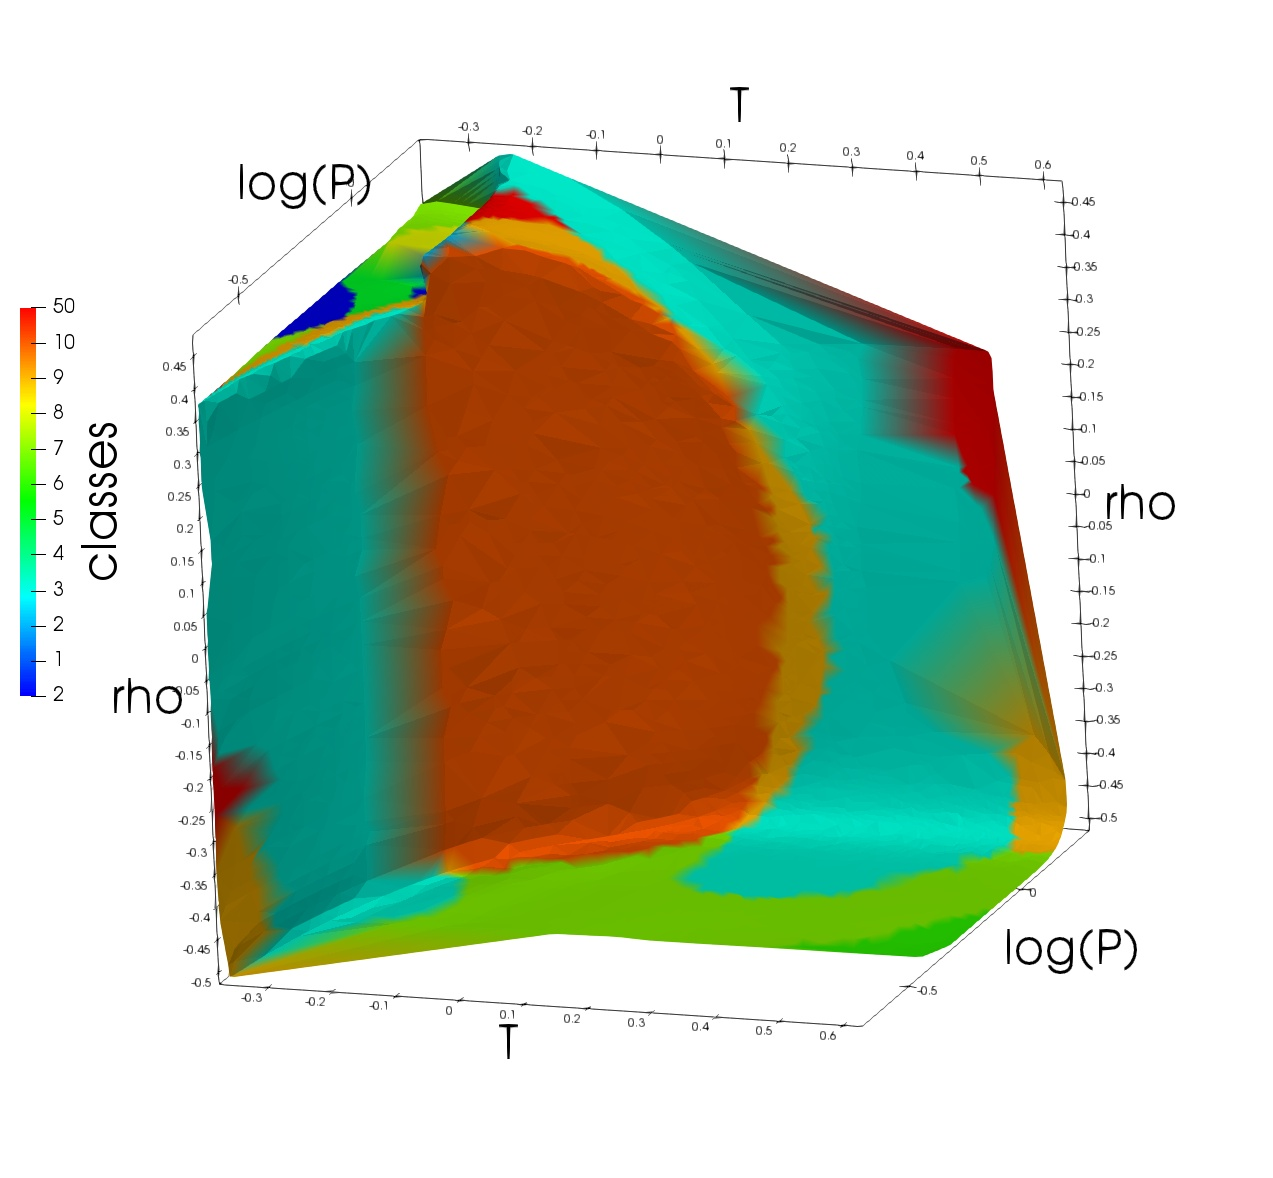
\includegraphics[width=3in]{../slides/classifier_good.jpg}
  \caption{\label{fig:classified}Result of the unsupervised phase
    classifier. Compare this plot to the original labeled dataset
    Figure \ref{fig:pTrho}. Note the axes are in the
    nondimensionalized scaling.}
\end{figure}

\hypertarget{header-n3321}{%
\section{Simulation}\label{header-n3321}}

Examining the $T,p,\rho$ surface allows for human interpretability, but
the decoder actually yields four new functions with two unknowns:
$D(q)=\{T(q),p(q),\rho(q),h(q)\}$. These surfaces can be plotted as
independent 2D functions: the surface of \ref{fig:classified} is
unfolded into the new parameterization in Figure \ref{fig:foursurfaces}.
\begin{figure}
  \centering
  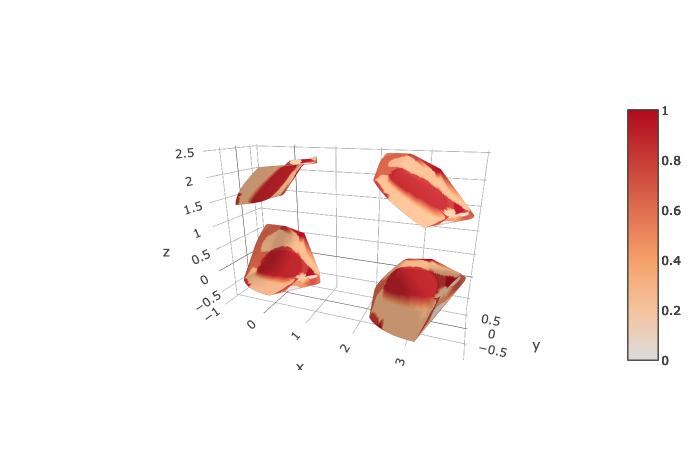
\includegraphics{../slides/water_four_surfaces_plot.png}
  \caption{\label{fig:foursurfaces}The four 2D surfaces that make up
    the new parameterization. The learned surface captures the sharp
    kinks and vertical fronts in Figure \ref{fig:classifyingresult},
    but is an analytic and smooth function of the two learned unknowns.}
  \end{figure}

With the trained model, we solve for \(q_1(t)\) and \(q_2(t)\) such that:
\begin{align}
\partial_t \rho(q_1,q_2) & = \mathbf{k} \left( p_\infty-p(q_1,q_2) \right)  + r \\
\partial_t \left(\rho h(q_1,q_2)-p\right) &
                                            =\mathbf{k}_T(T_\infty-T(q_1,q_2))  + s + \frac{\rho h}{h}\left(\mathbf{k}_p(p_\infty - p) + r\right)
\end{align}
where the expressions for  \(\rho(q_1,q_2)\) etc. are the back of the
trained autoencoder,. The trained
autoencoder automatically removes the local constraint, satisfying
\begin{equation}
eos(D(q_1,q_2)) = 0 \, \forall \,q_1,q_2
\end{equation}
Thus, the system will always satisfy the constraints as $q$ is
evolved, even during intermediate iterative solution steps. Note again
that the balance laws are directly incorporated into the simulation
after loading the trained model.

To develop the rest of the discretization, we introduce the compact form:
\begin{align}
\partial_t m(T,p,\rho,h) &= r(T,p,\rho,h)\\
eos(T,p,\rho,h) &= 0
\end{align}
where $m=\{\rho,\rho h -p\}$ and $r$ is the right hand side, where
$eos(T,p,\rho,h)=0$ is the material constraint.


The decoder part of the network is inserted into the balance law
\begin{equation}
\partial_t (D(q)) = r(D(q))
\end{equation}
We can parameterize this equation with any time stepping scheme, .e.g. a
Runge-Kutta scheme. For subsurface flow, backward Euler is popular due
to its simplicity and L-stability, which we follow since the topic of
this paper is not exploring new time stepping schemes. This yields the
discretized algebraic equation for \(q_i\) and \(t+\Delta t\) given the
value \(q^0\) at \(t\),

\begin{equation}
0 = R(q^i) = m(q^{i}) - m(q^{0}) - \Delta t \, r(q^i)
\end{equation}
where we have called the equation \(R(q)\). By design \(R(q)\) is smooth
enough to solve with Newton's method without any statemachine logic:
\begin{equation}
\frac{\partial R}{\partial q} \Delta q^{k+1} = - R(q^k)
\end{equation}
with the update
\begin{equation}
q^{k+1} = q^k + \alpha\Delta q^{k+1}
\end{equation}
where $\alpha$ is an under relaxation parameter.

This equation is deceptively simple: the function $R(q)$ has complex logic encoded in it; if-then
statements appear if the model used activations such as rectifiers.
However, the complex material behavior which traditionally requires
the vast majority of programming was implemented automatically by the
models; implementing equations XX, XX, and XX requires only a few lines
of human-written code. 

\subsection{Dimensionalization}

Recall that the datasets are normalized to be zero-center and
unit-ranged to improve training. Thus, the outputs of the decoder are not in true
units.
The ranges are saved in a separate file which are loaded by the
simulation. The network is loaded, the $D(q)$ is extracted, and the following
transformations are applied to the outputs:
\begin{align}
T(q)      &= \left(T_{max}-T_{min}\right) D_T(q) +T_{mean} \\
p(q)      &= \exp\left(\left( p_{max}-p_{min}\right)
            D_p(q) +p_{mean} \right) \\
\rho(q) &= \left(\rho_{max}-\rho_{min}\right) D_{\rho}(q) +\rho_{mean}\\
\rho h(q)      &= \left(\rho h_{max}-\rho h_{min}\right) D_h(q)  + \rho h_{mean}
\end{align}
The exponent transformation is only applied to the cases where
$\log(p)$ was used to make the training set.
The range values are in the proper units, so that equation rows in the
simulation are in SI units.


\hypertarget{header-n3339}{%
\subsection{Initialization}\label{header-n3339}}

There is a caveat with representing the degrees of freedom of the system
on a learned space: the user does not know the meaning of $q$ as an
input. Further, the values of $q$ vary from network to network and
depend on the parameterization. The user needs to be able to specify the
"real" physical quantities.

Since the original manifold is 2D, the user only needs to specify two
initial values. In a multiphase solver such as TOUGH, the state needs
to be specified with the two primary variables plus the state tag (sans input file formatting): 
\begin{verbatim}
    9e5 20 Aqu
    0.4 20 AqG
\end{verbatim}
Note that the first primary variable means pressure in the first line
for a pure-liquid state,
but saturation in the second line for the liquid-gas equilibrium.
This makes sense to human intuition but
still leads to bugs and occasionally requires looking up values in
textbooks or the software manual. (Is it $S_{gas}$ or $S_{aqu}$ on the second
line?) A fully fledged solver needs to check the user specified
initial conditions for erroneous inputs, but it cannot detect ambiguities.

The extra process of determining the initial state means that more error checking is needed
in verifying user inputs, but this is necessary in any
multiphase/multicomponent reservoir simulator. LatentSim does not yet
detect and report errors, and only reports divergence. In our study, the
testing problem specifications are all correct, but not all network
realizations are acceptable. Failure to determine a \(q\) for one of the
test initial conditions is a common mode of detecting unacceptable
network realizations; this is marked as a testing error during training
which invalidates a model as a potential realization.

The current implementation LatentSim does not support inputting via
saturations on the equilibria, a commonly used primary variable, but
this problem could be solved with future engineering work for a
non-experimental simulator.

For LatentSim, the input system is not yet as robust as a
fully-fledged user-facing simulator, but the inputs are specified in
the $T p \rho h$ space instead of the $q$ space.
The user (or test problem) specifies any two of the four values in a
dictionary format,
\begin{verbatim}
    p=9e5 T=20
    rho=500 T=20
\end{verbatim}
Then, the simulator must determine $q(t=0)$ from these two
values, but the econder only works when all four values are on the
surface. Let $s=\{T,p,\rho,\rho h\}$ be a four dimensional
variable of the stacked physical quantities. It is necessary to
actually solve the following nonlinear problem
on the decoder for the indices $i$ of the two specified values:
\begin{equation}
  D(q^0)_i = s^0_i \quad \text{for specified}\; i
\end{equation}
This equation has two rows indexing into the four state variables;
e.g. only the rows associated with $p$ and $T$ are solved if those are
specified, which is usually the case. The resulting system of
equations is solved with Newton's method. The two corresponding rows are cut out of
the tangent matrix to $D$,
\begin{equation}
K_{ij} = \frac{\partial D_i}{\partial q_j}  \quad \text{for
    specified}\; i, \text{for}\;j=1,2
\end{equation}
and the $2\times2$ linear system is solved for an update to $q$,
\begin{equation}
K_{ij}\Delta q_j = s^0_i-D(q)_i
\end{equation}
The iteration on $q$ is repeated until convergence, with under-relaxation used again to update:
 \begin{equation}
q^0_{k+1} =q^0_{k} + \alpha \Delta q_{k}
\end{equation}
with the under-relaxation parameter that is usually set to $\alpha \approx
0.1$.

The initial condition problem is not guaranteed to converge, however,
and often does not.
For example, if the initial guess was in the liquid phase and the target point
in the EOS space is in a solid, the iteration will fail.
To address this issue, we perform multiple starts with an initial condition in each
phase and equilibrium, discard points that diverge, and then pick the
\(q\) that is closest to the two specified components. The multiple
start points are specified at EOS development time to form a set of
values that represent middle points for each phase,
\begin{equation}
\left\{s_{guess}\right\} = \left\{ \left(\begin{array}{c}
\bar{T}_{gas}\\
\bar{p}_{gas}\\
\bar{\rho}_{gas}\\
\bar{\rho h}_{gas}
\end{array}\right),\left(\begin{array}{c}
\bar{T}_{liq}\\
\bar{p}_{liq}\\
\bar{\rho}_{liq}\\
\bar{\rho h}_{liq}
\end{array}\right),\left(\begin{array}{c}
\bar{T}_{ice}\\
\bar{p}_{ice}\\
\bar{\rho}_{ice}\\
\bar{\rho h}_{ice}
\end{array}\right)... \right\}
  \end{equation}
The multistart method could be specified without any prior knowledge
with random points, but this is a sufficiently robust method for
now. Each of the possible guess points is used to fill in the two
unspecified values as guesses and then passed into the encoder.
E.g. if $p$ and $T$ were specified, each possible $\bar{\rho}$ and
$\bar{h}$ combination from the above sets are filled in to provide
multiple guesses for $q$,
\begin{equation}
s^0 = \left(\begin{array}{c}
T^*(0)\\
p^*(0)\\
\bar{\rho}_{guess}\\
\bar{h}_{guess}
\end{array}\right);\quad q^0_{guess}=E\left(s^0\right)
 \end{equation}
 These sets of $q^0_{guess}$ are then iterated upon using the Newton's
 method procedure. 

It is further possible that none of the initial guesses for this iteration
converge. There are two possibilities: the target state point is
incorrectly specified or out-of-range (e.g., negative density), or the
network is incapable of representing the desired material properties
(i.e., poorly trained). The first possibility shows an invalid
problem specification for the chosen EOS. The second possibility is
crucial to the automated training process. If a given network cannot
find an initial condition for every possible test problem, it fails
the tests and is marked as invalid. This is one way of automatically
verifying the training process.


\hypertarget{header-n3493}{%
\subsection{Methodology Summary}\label{header-n3493}}

\begin{enumerate}
\def\labelenumi{\arabic{enumi}.}
\item
  Make a database of \(T,p,\rho,\rho h, ,...\)
  \begin{itemize}
  \item
    Piece together empirical fits for each phase from literature
  \item
    (\emph{Experimental data in the future})
  \end{itemize}
\item
  Normalize (and \(\log(p)\)) the database, shuffle it

  \begin{itemize}
  \item
    \(\log(p)\) distributes the low-\(p\) phases evenly w.r.t.
    high-\(p\) phases
  \end{itemize}
\item
  Train the autoencoder on batch-generated architectures. Note that
  phase labels are not used.
\item
  Load the models and generate physics code
\item
  Verify and grade architectures on tests

  \begin{itemize}
  \item
    Need more than autoencoder mean-squared-error
  \item
    Differentiability and numerical stability in simulation
  \item
    Evaluation speed (billions of times in a simulation!)
  \end{itemize}
\item
  Pick best one to package into production code
\end{enumerate}

\begin{figure}
  \centering
  \includegraphics[width=6in]{../figures/workflow_vector.pdf}
  \caption{\label{fig:workflow}Work flow of the simulation programming process.}
\end{figure}
This process yields are more complicated simulation software system
than previous generations. The architecture and workflow from problem
specification to user experience is illustrated in Figure
\ref{fig:workflow}.
Previous generations of simulators were entirely composed of human
written computer code, with some inline parameters (such as those of
the IAPWS fits typed into constants in dedicated fortran files)
fits and the occasional parameter files that are fed into the system
as inputs (such as reaction rates databases.)
Now, the behavior of the software is not only defined by the human
written code, it is also defined by the model it loads, and the
dataset that produced it.

In our vision, the theoretician or experimentalist specify a dataset
defined the possible states of the material. Multiple architectures
are trained using the autoencoder unsupervised representation learning
goal. Then, the simulation is ran by loading in each of the models and tested against known problems that
span the problem space. Some of the tests are written by the original
developers, and some of them must be specified by the scientist to
pass through the newly added physical regimes.
This testing process detects models that may have faired well in the
ML process and produced low values of the loss function on testing and
validation, but cannot be actually used in the simulation.
This testing process is also used to determine the model that is
optimal in terms of compute time and satisfactorily accurate.
The ``best'' model can then be ``shipped'' (i.e., marked for
deployment in DVC) to be automatically selected by the final end user,
who only specifies the Equation of State.

What is not shown in this figure is the testing of the data, and the
testing of the simulation framework, which are needed in a
fully-fledged machine learning based software system \cite{google ML smells}.
Testing of the data is performed before the simulation
methodology. These are contained in the Equations\_Of\_State package in our case, and would
need to be performed by the theoretician and experimentalist feed-side
users.
Integration testing of the train-deploy-load-simulation framework is
performed using the linear equation of state as a trivial test dataset
with a trivial linear model. 

\begin{algorithm}
  \caption{Psuedo code of the simulation}
\begin{verbatim}
specify EOS and a which network
load network from database
build DAE graph
input problem properties and initial value
solve for q0: D(q0) = s0
loop t=0 to t_max:
    solve for q[i]: R(q[i],q[i-1])=0
    decode s[i] = D(q[i])
\end{verbatim}
  \end{algorithm}

\hypertarget{header-n3356}{%
\section{Architecture}\label{header-n3356}}

The use of ML models yields a new software structure paradigm. It is now much simpler to implement new equation of state modules in
the simulation package, but managing the datasets and models adds
another layer to the software management. The high-level architecture
and low-level implementation details developed for the prototype
LatentSim are described in this section.

LatentSim is implemented entirely in Python 3 using the 

The original datasets are written out as .csv files. To prep the
datasets, the numbers are scaled to a zero-centered unit-range, shuffled, and broken up into the
2/3-1/6-1/6 subdivisions for train, test, and validate subsets. The
sets are stored as simple .npy files, with an accompanying short csv file
for the scaling (which is loaded by the simulation to de-scale the
network outputs.)


The ``hub'' has a directory structure:
\begin{verbatim}
  1. training\_[EOS]
    - One folder per architecture
      - MonitoredTraningSession checkpoints
      - Tensorboard summaries
      - .csv 3d plot renderings
    - More architectures...
  2. training\_[other EOS]...
  3. test\_database
    - One sqlite file per EOS containing all tests
  4. report
    - static renderings (superseded by Dash app)
\end{verbatim}
The code has the following structure:
\begin{verbatim}
  1. sources for data
  2. prepped data\_files
  3. reference solutions for testing
  4. training code
  5. LatentSim.py
  6. testing code
  7. Dash app
\end{verbatim}
For every EOS, there are multiple generated implementations.
After using a combination of Tensorboard, [] Visdom, [] and Paraview [] during
development, a custom Dash [] web interface was ultimately developed
to asses the results. A screenshot interface is shown in Figure []. The
interface allows the developer (i.e., the author) to browse all
statistics, renderings, of the trained surfaces and their test
problems.

In the version of the software distributed to users, only one
``frozen'' and optimized model needs to be included per equation of state.

\subsection{Implementation details}

The training framework and simulations are implemented in TensorFlow 
using custom defined operations. The various visualizations are built
using Matplotlib, Plotly, and Visdom. The accompanying video was
generated using Paraview.

The codebase is released open source at
\url{https://github.com/afqueiruga/latentsim}. Datasets and other
presentation artifacts such as videos and interactive plots are stored
in git-lfs. Helper methods and
custom optimizers that the
author reuses in various TensorFlow-based projects are factored out in
the dully-named \url{https://github.com/afqueiruga/afqstensorflowutils}.
The implementation of the empirical equations of state for water are
factored out at
\href{https://github.com/afqueiruga/equations_of_state}{https://github.com/afqueiruga/equations\_of\_state}.

\subsection{Things we'll do differently}

Adopt julia for at least the simulation



\hypertarget{header-n3359}{%
\section{Simulation Evaluation}\label{header-n3359}}

Multiple hyperparameters are trained.

Each architecture trained on the autoencoder task is then

The phase space of water is broken up into three different extents to
change the complexity of the training process:

\begin{enumerate}
\def\labelenumi{\arabic{enumi}.}
\item Linear Equation of State: the range is $ p = 10^5+[-10^3, 10^3]
  Pa,\quad T = [ 19, 21 ] ^o C$. This reduces to the single phase
  Darcy's law problem where the material has constant compressibility
  and heat capacity. This is the most basic test of the training
  framework, and provides analytical solutions to test the simulation
  framework.
\item Liquid-Gas Regime: the range is  $ p = [100,5\times 10^5] Pa,
  \quad T = [274,594] K$. This restricts the domain to only one phase
  boundary. With this range, it is possible to find a linear
  combination of $T,p,\rho,h$ that can make a 1-1 mapping. (The usual
  $T-p$ combination does not, but $\rho-h$ would.)
\item Solid-Liquid-Gas-Supercritical Regimes: this covers the full
  extent of the parameterized equation of state of water,
    $ p = [6\times 10^{-6},3\times 10^8]Pa, \quad T = [150,1000] K
    $. This problem has no linear mapping to a unique latent space.
\end{enumerate}


\hypertarget{header-n3418}{%
\subsection{Validation and Testing}\label{header-n3418}}

The verification problems are listed in Table \ref{tab:problems}.
\begin{table}
  \caption{\label{tag:problems}Enumeration of the problems used to test and evaluate each fo the generated architectures}
\begin{tabular}{l|c|c|c}
  Name & start & path & end\\
\hline
\end{tabular}
\end{table}


The linear problem is only of interest for integration testing. Only one
hyperparameter set for each architecture-generating class was trained
on the dataset. The simulation code is then executed on the two linear
problems, verifying the implementation of the multi-stage process and
generation of the balance laws. In a fully-fledged simulator including flow, this
dataset would yield a two-phase Darcy's law equation of state, which
would allow for verifcation against that set of analytical solutions.

The simulator was benchmarke against the long standing TOUGH+ multiphase
multicomponent simulator. Single-grid block simulations were set up for most of the cases. TOUGH+
does not handle supercritical \ch{H2O}, so these test problems were not
used to benchmark. (The supercritical phase region is not practically
relevant for water, but it is very important for other fluids such as
\ch{CO2}.) (Note that, as a major motivation of this work, adding
supercritical states to the existing Fortran simulator would require
coding of one new logical state with two new state transitions with
primary variable switches; for the approach of this paper, the dataset
just needed to be extended.)


\hypertarget{header-n3421}{%
\section{Conclusions}\label{header-n3421}}

\begin{itemize}
\item
  Deep learning to replace and improve hand-baked equations and
  algorithms
\item
\item
  \textbf{Only training the material representation, not the balance
  laws}
\item
  Extend to more complicated materials
\item
  Put into a flow simulation
\item
  Close loop on testing with reinforcement learning
\end{itemize}

The ultimate goal for this work is to automate integration of data
analysis into simulation.

We hypothesize this end-to-end approach will allow the system to develop
\emph{better} simulations \emph{faster}.

We demonstrated a specially crafted architecture whose parameters can be
human interpretted and perform unsupervised phase/equilibria
classification.

We illustrated a programming model that is able to incorporate machine
learning models into existing well known computational methodologies.
This allows us to enforce physically known quantities, such as the
balance laws.

The TensorFlow system is not quite suited for this type of workflow -\/-
the resulting simulations are extremely slow due to repeated calls to
session.run and a very complicated graph structure for the polynomials.
Currently, the system is being reimplemented in Julia using Flux and
Zygote to seamlessly reincorporate into a fully-fledged new reservoir
simulator. The pendulum has been reimplemented in Julia at .

We are also demonstrating a new programming paradigm applied to
scientific computing. The entire system has another level of complexity
to it. An offline training phase searches for a new representation, i.e.
for new equations with new unknown degrees of freedom, that are good to
solve.

Each implemented equation of state (three options in this work spanning
different extents of \ch{H2O}) has a database of potential realizations.
The entries are model architectures, parameters, and training
environment configurations and logs for each equation-of-state dataset.
This database of models replaces a version controlled repository of user
written modules. Hundreds of trials for novel primary variable
configurations happen in a matter of minutes on a workstation in place
of pain-staking trial-and-error labor performed with human "intuition"
and experience. We did encode a little bit of human intuition into the
model architectures and tricks for initializing the networks.

We can also think about this work as offline preconditioning.

In TOUGH, for one instance, all of the calculations are performed in SI units because it is simply too much labor to normalize everything! Adverse effects to iterative algorithms and floating point error propagation occur, especially because numerical differentiation is used.
The learned primary variables are normalized to a unit range around zero, and the scaling matrix is explicitly in one step. The scaling matrix could be a way to systematically non-dimensionalize the entire problem.

The larger simulation code links into the trained database to load the
computer-written model into the computation graph for the simulation,
deriving all needed ingredients for the mainloop using automatic
differentiation.

The simulation inputs are the name of the equation of state, .e.g,
``water\_lg'' or ``water\_slgc'', and the name of the architecture
hyperparameters, e.g. ``Classifying\_pT\_1.0\_1,3,6,12,Sigmoid''.
In a mature code, the name of the architecture loaded would be hidden
from the end-user and would be a setting which the doman scientist and developer freezes
after checking the training process.

Techniques such as L1 regularization would be needed to search for low
cost models that also satisfy our desire for Occam's razor
simplifications. (The IAPWS relations used a preliminary form of this
type of simplification, but are not optimal in the author's opinion.)

A fully automated testing system can verify which realizations worked
(relate this to an independent review board comparing the results the
independently developed codes) and then select the fastest and most
robust one.


In future work, we would want to continue appending new \(q\)s in a
systemic way to derive, e.g., an \(H_2O + NaCl\) equation of state with
3 degrees of freedom, bootstraping from the pre-trained \(H_2O\)
architecture with 2 degrees of freedom.

\section*{Acknowlegements}
%\acks

This work was supported by Department of Energy, Office of Fossil
Energy contracts
1. Hydrates
2. Shales

The author would like to thank his colleagues Matt Reagan and George
Moridis for all their instruction on chemsitry. 
\bibliographystyle{plainnat}
\bibliography{zotero}

\end{document}
